\subsubsection{Markov Decision Process}
The interaction of a learner to achieve a goal can be modeled mathematically through a \textit{Markov Decision Process} (or \textit{MDP}). This allows statements about learning algorithms to be theoretically proven, such as the convergence of an agent's policy to its optimum. \cite{sutton}

We start by defining that the learning and acting instance is called the \textit{agent}, whereas its surroundings, which are delivering situations, responding to the agents actions and controlling the reward signal, are called the \textit{environment}. The agent therefore strives to maximize its rewards by performing actions based on previously perceived situations. \cite{sutton}

In Markov Decision Processes, the agent-environment interaction only occurs on discrete timesteps $t \in \{0, 1, 2, ...\}$. At each timestep $t$, the environment provides a \textit{state} $S_t \in \mathscr{S}$ to the agent, where $\mathscr{S}$ is the set of all possible states. Based on this state, the agent may select an \textit{action} $A_t \in \mathscr{A}(S_t)$, with $\mathscr{A}(S_t)$ being the set of legal actions in state $S_t$. As a result of this action, the agent receives a \textit{reward} $R_t \in \mathscr{R} \subset \mathbb{R}$. Note that this means there is no reward associated with the very first timestep. A sequence following this pattern of states, actions and rewards is called a \textit{trajectory}. This process is visualized in figure \ref{fig:mdp_visualization}. \cite{sutton}

\begin{figure}[h]
    \centering
    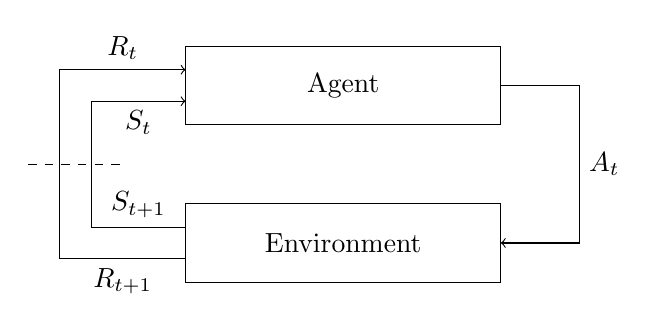
\begin{tikzpicture}
        \draw (0, 2) rectangle node {Agent} (4, 3);
        \draw (0, 0) rectangle node {Environment} (4, 1);

        \draw [->] (4, 2.5) -- (5, 2.5) -- node[right] {$A_t$} (5, 0.5) -- (4, 0.5);

        \draw [->] (0, 0.3) -- node[below] {$R_{t+1}$} (-1.6, 0.3) -- (-1.6, 2.7) --node[above] {$R_t$}  (0, 2.7);
        \draw [->] (0, 0.7) -- node[above] {$S_{t+1}$} (-1.2, 0.7) -- (-1.2, 2.3) -- node[below] {$S_t$} (0, 2.3);

        \draw [dashed] (-2, 1.5) -- (-0.8, 1.5);
    \end{tikzpicture}
    \caption{Visualization of the feedback loop in a Markov Decision Process.}
    \label{fig:mdp_visualization}
\end{figure}

An agent should not focus solely on choosing the action $A_t$ which results in the highest \textit{immediate reward} $R_{t+1}$. Instead, future rewards should also be taken into consideration. Formally, we define the \textit{return}, which is the sum of all rewards at subsequent timesteps until the final timestep $T$.
\begin{equation*}
    G_t = R_{t+1} + R_{t+2} + R_{t+3} + ... + R_T
\end{equation*}
Accordingly, an agent aims to maximize the expected return at each step. The concept of a final timestep only applies for tasks which have a clearly defined beginning and end, i.e. are repetitive in nature. We call a single cycle of these repetitive tasks \textit{episode}. \cite{sutton}

For tasks which can potentially continue indefinitely, i.e. $T = \infty$, $G_t$ may also become infinite. To avoid this issue, we introduce a \textit{discount rate} (or \textit{discount factor}) $\gamma \in [0, 1]$, and define the \textit{discounted return} as follows:
\begin{equation*}
    G_t = R_{t+1} + \gamma R_{t+2} + \gamma^2 R_{t+3} + ...
        = \sum_{k=t+1}^T \gamma^{k-t-1} R_k
\end{equation*}
The parameter $\gamma$ determines to what extend the agent prefers rewards in the near over those in the far future. As an example, an agent with $\gamma = 0$ cares only about the immediate reward, whereas the same agent with $\gamma = 0.99$ will optimize for a large time window of rewards. Choosing $\gamma < 1$ ensures that $G_t$ will not become infinite. \cite{sutton}